
\section{IARU-Bandplan für 70 cm}
\label{section:iaru_bandplan_70cm}
\begin{frame}%STARTCONTENT

\begin{figure}
    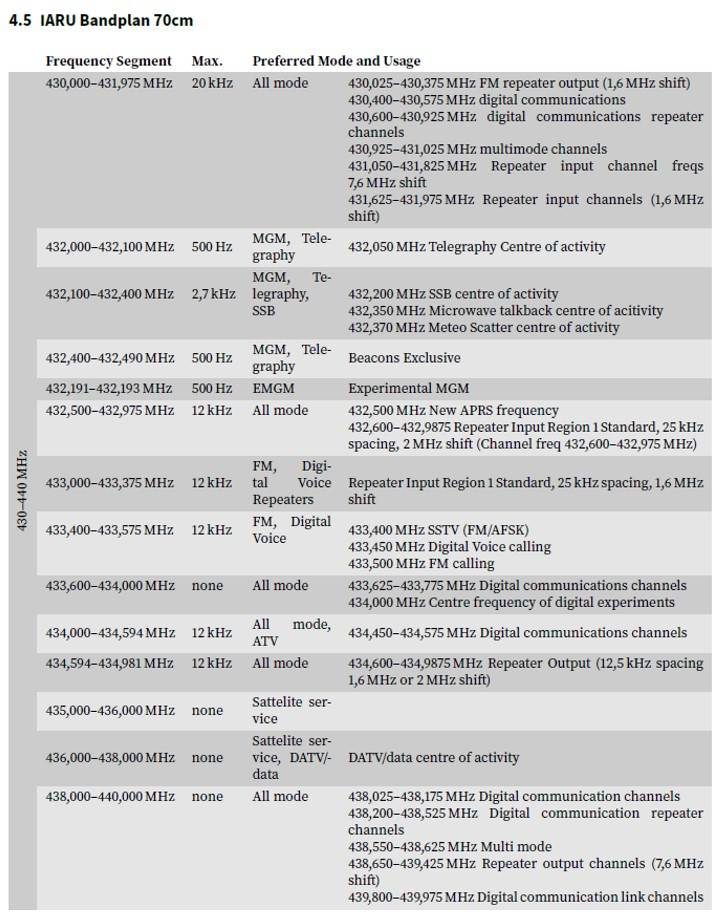
\includegraphics[width=0.85\textwidth]{foto/103}
    \caption{\scriptsize IARU-Bandplan \qty{70}{\centi\metre}}
    \label{n_iaru_bandplan_70cm}
\end{figure}

\end{frame}

\begin{frame}
\only<1>{
\begin{QQuestion}{BC206}{Welche Frequenz empfiehlt der IARU-Bandplan für einen allgemeinen Anruf mit analoger FM-Telefonie im \qty{70}{cm}-Band?}{\qty{433,450}{\MHz}}
{\qty{433,500}{\MHz}}
{\qty{432,500}{\MHz}}
{\qty{432,050}{\MHz}}
\end{QQuestion}

}
\only<2>{
\begin{QQuestion}{BC206}{Welche Frequenz empfiehlt der IARU-Bandplan für einen allgemeinen Anruf mit analoger FM-Telefonie im \qty{70}{cm}-Band?}{\qty{433,450}{\MHz}}
{\textbf{\textcolor{DARCgreen}{\qty{433,500}{\MHz}}}}
{\qty{432,500}{\MHz}}
{\qty{432,050}{\MHz}}
\end{QQuestion}

}
\end{frame}

\begin{frame}
\only<1>{
\begin{QQuestion}{BC208}{Welche Frequenz empfiehlt der IARU-Bandplan für einen allgemeinen Anruf mit digitaler Telefonie im \qty{70}{cm}-Band?}{\qty{433,500}{\MHz}}
{\qty{433,450}{\MHz}}
{\qty{432,500}{\MHz}}
{\qty{432,050}{\MHz}}
\end{QQuestion}

}
\only<2>{
\begin{QQuestion}{BC208}{Welche Frequenz empfiehlt der IARU-Bandplan für einen allgemeinen Anruf mit digitaler Telefonie im \qty{70}{cm}-Band?}{\qty{433,500}{\MHz}}
{\textbf{\textcolor{DARCgreen}{\qty{433,450}{\MHz}}}}
{\qty{432,500}{\MHz}}
{\qty{432,050}{\MHz}}
\end{QQuestion}

}
\end{frame}

\begin{frame}
\only<1>{
\begin{QQuestion}{BC212}{Welche Frequenz bzw. welchen Frequenzbereich sieht der IARU-Bandplan als Aktivitätszentrum für SSB-Telefonie im \qty{70}{cm}-Band vor?}{\qty{434,000}{\MHz}}
{\qty{432,200}{\MHz}}
{\qtyrange{432,600}{432,9875}{\MHz}}
{\qtyrange{434,450}{434,575}{\MHz}}
\end{QQuestion}

}
\only<2>{
\begin{QQuestion}{BC212}{Welche Frequenz bzw. welchen Frequenzbereich sieht der IARU-Bandplan als Aktivitätszentrum für SSB-Telefonie im \qty{70}{cm}-Band vor?}{\qty{434,000}{\MHz}}
{\textbf{\textcolor{DARCgreen}{\qty{432,200}{\MHz}}}}
{\qtyrange{432,600}{432,9875}{\MHz}}
{\qtyrange{434,450}{434,575}{\MHz}}
\end{QQuestion}

}
\end{frame}

\begin{frame}
\only<1>{
\begin{QQuestion}{BC221}{Warum sollten Sie auf \qty{435,500}{\MHz} \underline{keine} Direktverbindung in FM-Telefonie zu einem Funkamateur aufnehmen, der sich im Nachbarort befindet? Der IARU-Bandplan empfiehlt diesen Bereich für die Nutzung durch~...}{Satellitenfunk.}
{Repeater.}
{Morsetelegrafie und schmalbandige digitale Übertragungsverfahren.}
{Baken.}
\end{QQuestion}

}
\only<2>{
\begin{QQuestion}{BC221}{Warum sollten Sie auf \qty{435,500}{\MHz} \underline{keine} Direktverbindung in FM-Telefonie zu einem Funkamateur aufnehmen, der sich im Nachbarort befindet? Der IARU-Bandplan empfiehlt diesen Bereich für die Nutzung durch~...}{\textbf{\textcolor{DARCgreen}{Satellitenfunk.}}}
{Repeater.}
{Morsetelegrafie und schmalbandige digitale Übertragungsverfahren.}
{Baken.}
\end{QQuestion}

}
\end{frame}

\begin{frame}
\only<1>{
\begin{QQuestion}{BC222}{Warum sollten Sie auf \qty{439,200}{\MHz} \underline{keine} Direktverbindung in FM-Telefonie zu einem Funkamateur aufnehmen, der sich im Nachbarort befindet? Der IARU-Bandplan empfiehlt diesen Bereich für die Nutzung durch~...}{Morsetelegrafie und schmalbandige digitale Übertragungsverfahren.}
{Satellitenfunk.}
{Repeater.}
{Baken.}
\end{QQuestion}

}
\only<2>{
\begin{QQuestion}{BC222}{Warum sollten Sie auf \qty{439,200}{\MHz} \underline{keine} Direktverbindung in FM-Telefonie zu einem Funkamateur aufnehmen, der sich im Nachbarort befindet? Der IARU-Bandplan empfiehlt diesen Bereich für die Nutzung durch~...}{Morsetelegrafie und schmalbandige digitale Übertragungsverfahren.}
{Satellitenfunk.}
{\textbf{\textcolor{DARCgreen}{Repeater.}}}
{Baken.}
\end{QQuestion}

}
\end{frame}

\begin{frame}
\only<1>{
\begin{QQuestion}{BC219}{Warum sollten Sie auf \qty{432,040}{\MHz} \underline{keine} Direktverbindung in FM-Telefonie zu einem Funkamateur aufnehmen, der sich im Nachbarort befindet? Der IARU-Bandplan empfiehlt diesen Bereich für die Nutzung durch~...}{Weltraumkommunikation.}
{Satellitenfunk.}
{Morsetelegrafie und schmalbandige digitale Übertragungsverfahren.}
{Baken.}
\end{QQuestion}

}
\only<2>{
\begin{QQuestion}{BC219}{Warum sollten Sie auf \qty{432,040}{\MHz} \underline{keine} Direktverbindung in FM-Telefonie zu einem Funkamateur aufnehmen, der sich im Nachbarort befindet? Der IARU-Bandplan empfiehlt diesen Bereich für die Nutzung durch~...}{Weltraumkommunikation.}
{Satellitenfunk.}
{\textbf{\textcolor{DARCgreen}{Morsetelegrafie und schmalbandige digitale Übertragungsverfahren.}}}
{Baken.}
\end{QQuestion}

}
\end{frame}

\begin{frame}
\only<1>{
\begin{QQuestion}{BC220}{Warum sollten Sie auf \qty{432,450}{\MHz} \underline{keine} Direktverbindung in FM-Telefonie zu einem Funkamateur aufnehmen, der sich im Nachbarort befindet? Der IARU-Bandplan empfiehlt diesen Bereich exklusiv für die Nutzung durch~...}{Satellitenfunk.}
{Baken.}
{Repeater.}
{Morsetelegrafie und schmalbandige digitale Übertragungsverfahren.}
\end{QQuestion}

}
\only<2>{
\begin{QQuestion}{BC220}{Warum sollten Sie auf \qty{432,450}{\MHz} \underline{keine} Direktverbindung in FM-Telefonie zu einem Funkamateur aufnehmen, der sich im Nachbarort befindet? Der IARU-Bandplan empfiehlt diesen Bereich exklusiv für die Nutzung durch~...}{Satellitenfunk.}
{\textbf{\textcolor{DARCgreen}{Baken.}}}
{Repeater.}
{Morsetelegrafie und schmalbandige digitale Übertragungsverfahren.}
\end{QQuestion}

}
\end{frame}%ENDCONTENT
